\chapter{Graphics}

There are two problems to consider here, how points on a grid are generated, and
how they are displayed. To generate points there needs to be a method of
procedural generation, i.e. creating an algorithm that can given a set of
parameters tell me where a point should or shouldn't be and what other points it
should or shouldn't connect to.

The problem of how they are displayed is another issue, how can we convey the
idea of moving through a space when the space is simply a grid? 

\section{Anatomy of the Work}
Viner's pen plotter work was created by a set of programs, created in
\verb|FORTRAN| using a set of subroutines called \verb|PICASO| (PIcture Computer
Algorithms SubroutineOriented) \citep{lycett_2016}, this was essentially a
line-drawing library, similar to what we are using processing / p5js for.
\verb|PICASO|'s use by Viner isn't well documented but the manual
\citep{picaso_manual} has many subroutines for transforming vertices according
to some rules. Some notes on Viner's work indicate there was definitely
mathematical thinking going on in the development.



\section{The Grid}
With the motif of the grid being the most obvious visible thing in Viner's art,
there needs to be a way to actually draw a grid to the screen; ideally each
vertex needs to be able to be separately controlled.

To do this I have adapted John Stell's work on Viner in his workshops
\cite{stell_unpublished}, using an object-oriented approach; but have created a
system where the grid is centred on a given \verb|x,y| coordinate. Essentially
there is a screen, and for every vertex at a column and row their relative
coordinates need to be calculated. This is simple with the following statement:


%the immediate issue here is that we want the grid to be drawn from the center out.
%How can we do this? A spiral? A space filling curve? We can't really
%have negative indicies to lists.
%
%Create a seperate notion of 'columns' and 'rows' that draw and x and y
%are infinite and inform what is to be rendered in those columns and rows
%
%How many columns and rows do we need? We define a grid size and it's n *
%that How do we map x and y to this notion? We have a grid size so we can
%work out how many are shown at a time, how to ensure that we are always
%in the center?  Perhaps this means we don't actually need to worry about
%where we are just what is rendered based on this. thus we let our x and
%y values determine what is immediately under us but the rest of the
%image renders around this

%for now at least I want to be able to draw points at a (x, y) dependant
%offset from the center of each point?
%
%center the grid on whatever x and y value we're at right now

\begin{center}
\begin{tabular}{c}
\begin{lstlisting}[language=java]
sx = (x + (gridSize * ((cols/2) - i)));
sy = (y + (gridSize * ((rows/2) - j)));
\end{lstlisting}
\end{tabular}
\end{center}

Where \verb|i,j| is the column and row value of the point, \verb|cols,rows|
are the total number of columns and rows, and \verb|gridSize| is the pixel size
of the grid (which is more of a guide than anything). The grid should also
be centred on \verb|x,y| so calling a translate before drawing any points should
be done:

\begin{center}
\begin{tabular}{c}
\begin{lstlisting}[language=java]
translate((width/2)+(0-x), (height/2)+(0-y));
\end{lstlisting}
\end{tabular}
\end{center}

All of this leads to a system where the centre point has a given coordinate and
we can find that coordinate for all other points around it, this also means we
can interpolate any parameters from the program to what should be expected at a
given coordinate; or we can also generate a terrain away from the main graphics
thread and draw them to the screen at a given coordinate.

\subsection{Demo}
Here a grid is prepared with fixed parameters that create distortion around
\verb|x=0, y=0|. This point is fixed, and when the program is interacted with
the world moves beneath the player rather than the point of distortion being
changed, the grid displayed is reflecting the `terrain' visible from the centre
point.

\begin{figure}[H]
\centering
\subfloat{\tikz[remember
picture]{\node(1AL){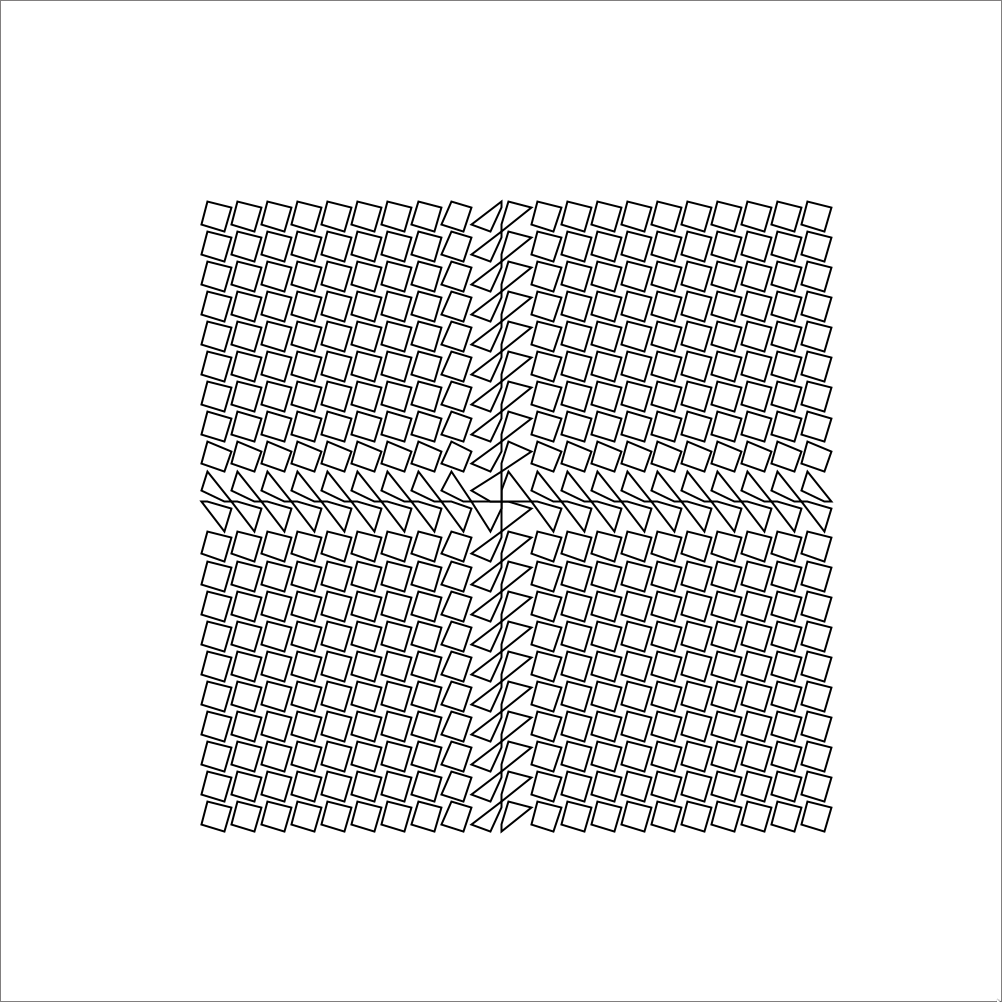
\includegraphics[width=.4\textwidth]{PoC3}};}}%
\hspace*{2cm}%
\subfloat{\tikz[remember
picture]{\node(1AR){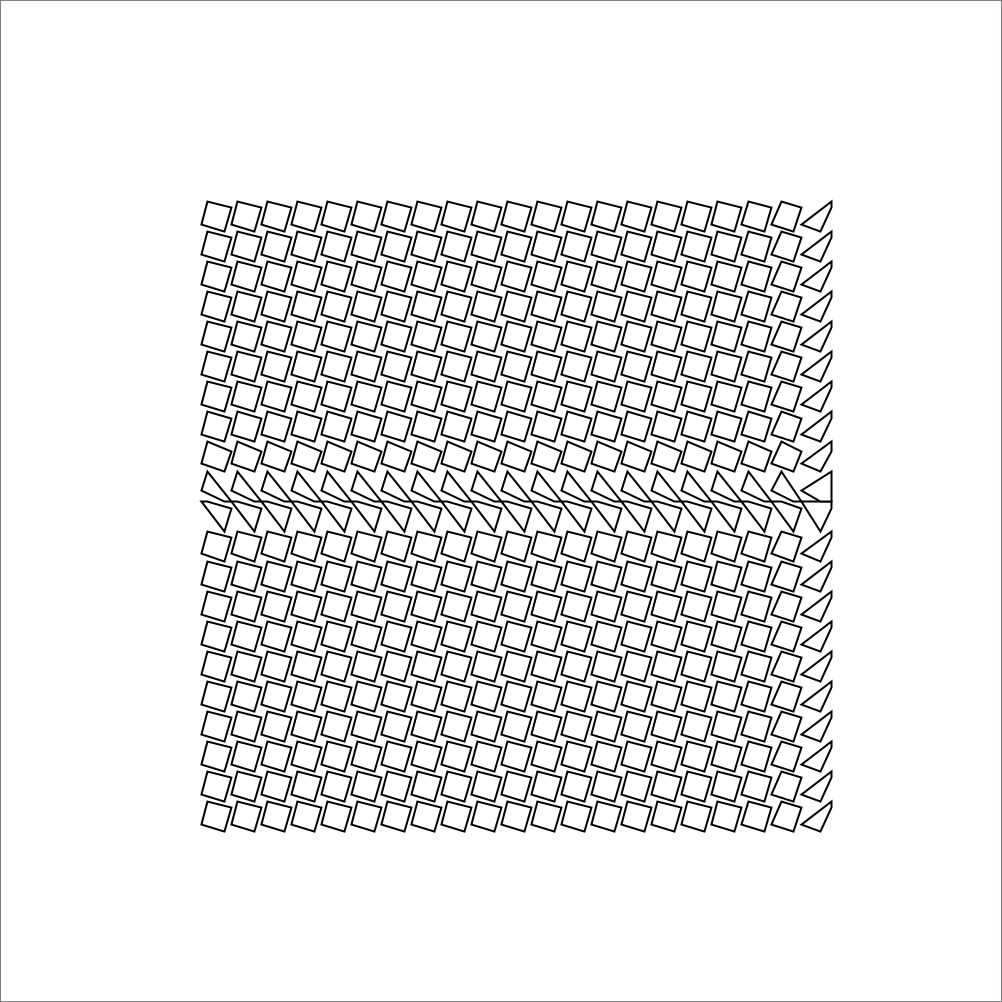
\includegraphics[width=.4\textwidth]{PoC2}};}}
\caption{The user presses `d' for a short time, increasing the `x' parameter}
\label{demomovement}
\end{figure}
\tikz[overlay,remember picture]{\draw[-latex,thick] (1AL) -- (1AL-|1AR.west)
node[midway,below]{};} 


\section{Landscape Generation}
% Talk about landscape analogy
The program should generate a `landscape' or `topology', this is an analogy for
a space that has an continuous change of the parameters across them. `Landscape'
is apt because we're exploring a set of features generated by the program much
like if you were to look at a topographic map. The user should have the feeling
of moving through a space like this, more than simply increasing some parameter
and immediately seeing a change throughout the grid.

% Talk about explorations into proc gen, dynamical systems etc.
This is the main question of how the program will work on a technical level, how
can we create an algorithm or mathematical model that explores the spaces that
Viner's work set out to create?

Dynamical systems may be of interest, and allow for a system to be created where
a state evolves into other states following some rules. These states can be
deterministic which is important for the objective that we have of recall, but
can also be chaotic, which may be aesthetically desirable.

Similarly, fractals may be useful for their self-similarity. Given we're working
with a grid, the ability to have self-similar properties may be considered to be
aesthetically useful.

%dynamical systems and fractals time


This leads to the choice between having each session using the software be
either random in some sense or the same every time. Ideally given a random
option to fulfil the ability to recall previous sessions, a seed would be given.
It seems then that the random choice contains the static choice and should be
the one to be carried out.
